\chapter*{ANTON-BIVENS-DAVIS 3.4 EJERCICIO 23}

\textbf{1)} Un satélite se encuentra en una órbita elíptica alrededor de la Tierra. Su distancia r (en millas) desde el centro de la Tierra está dada por$$r=\frac{4995}{1+0.12cos\theta}$$

donde $\theta$ es el ángulo medido desde el punto de la órbita más cercano a la superficie de la Tierra (ver la figura adjunta).
\begin{enumerate}[label=\alph*)]
	\item Halla la altitud del satélite en el perigeo (el punto más cercano a la superficie de la Tierra) y en el apogeo (el punto más alejado de la superficie de la Tierra). Usa 3960 mi como el radio de la Tierra.
	\item En el instante en que $\theta$ es 120°, el ángulo $\theta$ aumenta a una tasa de 2,7° /min. Halla la altitud del satélite y la tasa a la que cambia la altitud en ese instante. Expresa la tasa en unidades de mi/min.
\end{enumerate}

\begin{center}
	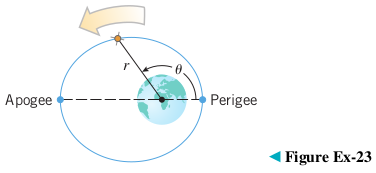
\includegraphics[height = 0.14\textheight]{recursos/image.png}\par
\end{center}


\text{a):} 1.-  Halla la altitud del satélite en el perigeo.\\
Tenenmos que evaluar la ecuación que nos da el radio del centro de la tierra al satélite, esto es cuado $\theta = 0$° pues en la trayectoria elíptica del satélite donde intersecta al eje horizontal en el punto más cercano a la tierra es el ángulo que se forma.
\begin{align*}
	r_{p} & =\frac{4995}{1+0.12cos\theta} \bigg|_{\theta=0} \\
	      & =\frac{4995}{1+0.12cos(0)}                      \\
	      & =\frac{4995}{1+0.12(1)}                         \\
	      & \simeq 4459.8214 \;mi                           \\
\end{align*}
Ahora para saber la altitud desde el punto más cercano a la superficie de la tierra al satélite debemos tomar en cuneta que $r_T=3960 \;mi$ para así calcular la diferencia de $r_p-r_T$, la cual nos dará la altitud deseada $$Altitud_p=r_p-r_T=4459.8214 \;mi-3960 \;mi\simeq 499.8214\;mi$$
$\therefore$ la Altitud del satélite en el perigeo es de $\simeq 499.8214\;mi$ de distancia.\\
2.- Repetimos el procedimiento en el punto más alejado, el apogeo, este caso ocurre cuando $\theta = 180$° pues considerando la trayectoria elíptica del satélite donde intersecta al eje horizontal en el punto más legano a la superficei de la tierra, el ángulo que se forma es de $180$°.
\begin{align*}
	r_{a} & =\frac{4995}{1+0.12cos\theta} \bigg|_{\theta=180} \\
	      & =\frac{4995}{1+0.12cos(180)}                      \\
	      & =\frac{4995}{1+0.12(-1)}                          \\
	      & \simeq 5676.1363 \;mi                             \\
\end{align*}
$5676.1363 \;mi$ es la distancia desde el centro de la tierra al satélite, debemos calcular la diferencia entre el radio de la tierra $r_T$ y la distancia en el punto $r_a$ para saber la altitud desde la superficie hasta el punto $r_a$$$Altitud_a = r_a-r_T=5676.1363 \;mi-3960\;mi\simeq 1716.1363 \;mi$$
$\therefore$ la Altitud del satélite en el Apogeo es de $\simeq 1716.1363 \;mi$ de distancia.\\
\textbf{b):} Halla la altitud del satélite y la tasa a la que cambia la altitud en el instante que $\theta$ es 120°.
Sabemos que el ángulo $\theta$ aumenta a una tasa de 2,7° /min. en ese instante.\\
1.- Para hallar la altitud del satélite debemos utilizamos el mismo argumento anterior cuando $\theta=120$°
\begin{align*}
	r_{s}     & =\frac{4995}{1+0.12cos\theta} \bigg|_{\theta=120} \\
	          & =\frac{4995}{1+0.12cos(120)}                      \\
	          & =\frac{4995}{1+0.12(-\frac{1}{2})}                \\
	          & \simeq 5313.8297 \;mi                             \\
	Altitud_s & = r_s-r_T                                         \\
	          & = 5313.8297 \;mi-3960\;mi                         \\
	          & \simeq 1353.8297\;mi
\end{align*}
$\therefore$ la Altitud del satélite cuando $\theta=120$° es de $\simeq 1353.8297\;mi$ de distancia.\\
la tasa a la que cambia la altitud en ese instante.

La altitud $r$ depende del ángulo $\theta$, y $\theta$ a su vez cambia con el tiempo $t$. La regla de la cadena nos permite relacionar estas tasas de cambio.
$$\frac{dr}{dt}=\frac{dr}{d\theta}\cdot\frac{d\theta}{dt}$$
\begin{multicols}{2}
	\noindent
	\begin{align*}
		\frac{dr}{d\theta}                          & =\frac{d}{d\theta}\left(\frac{4995}{1+0.12\cdot cos\theta}\right)                                 \\
		                                            & =-\frac{4995\cdot\left(-0.12\left(sen \theta\right)\right)}{\left(1+0.12\cdot cos\theta\right)^2} \\
		\therefore \frac{dr}{d\theta}               & =\frac{599.4\cdot\left(sen \theta\right)}{\left(1+0.12\cdot cos\theta\right)^2}                   \\
		\frac{d\theta}{dt}                          & = \frac{2.7^\circ}{min}                                                                           \\
		\text{Nota: en radianes }\frac{d\theta}{dt} & = \frac{2.7\cdot\pi}{180}
	\end{align*}
	\columnbreak
	\begin{align*}
		\implies\frac{dr}{dt}= & \frac{dr}{d\theta}\cdot\frac{d\theta}{dt}                                                                               \\
		=                      & \frac{599.4\cdot\left(sen \theta\right)}{\left(1+0.12\cdot cos\theta\right)^2}\cdot\left(\frac{2.7\cdot\pi}{180}\right) \\
		=                      & \frac{599.4\cdot\left(sen \theta\right)}{\left(1+0.12\cdot cos\theta\right)^2}\cdot\left(0.015\cdot\pi\right)           \\
		=                      & \frac{599.4\cdot\left(0.015\cdot\pi\right)\cdot\left(sen \theta\right)}{\left(1+0.12\cdot cos\theta\right)^2}           \\
		=                      & \frac{8.991\pi\cdot\left(sen \theta\right)}{\left(1+0.12\cdot cos\theta\right)^2}                                       \\
	\end{align*}
\end{multicols}
\vspace{-30px}
\begin{align*}
	\implies\frac{dr}{dt}\bigg|_{\theta=120^\circ}= & \frac{8.991\pi\cdot\left(sen (120^\circ)\right)}{\left(1+0.12\cdot cos(120^\circ)\right)^2}    \\
	=                                               & \frac{8.991\pi\cdot\left(\frac{\sqrt{3}}{2}\right)}{\left(1+0.12\cdot (-\frac{1}{2})\right)^2} \\
	\simeq                                          & \frac{24.4618}{0.8836}                                                                         \\
	\simeq                                          & 27.6842\;mi/min                                                                                \\
\end{align*}

$\therefore$ la tasa a la que cambia la altitud en ese instante es de $27.6842\;mi/min$
